% !TEX root = ./arock_pkg_main.tex
\section{Architecture}
The goal of the ARock package is to build an abstract framework to simplify the implementation of async-parallel algorithms. ARock reduces each application to the fixed-point problem \eqref{eqn:fix_point_set} with the fixed-point operator $\cT$ being CF. The operator $\cT$ can be a single stand along operator or formed by combination of multiple CF operators under certain operator splitting scheme. Then the ARock kernel takes the operator $\cT$ and runs the Algorithm \ref{alg:asyn_core} with a given number of workers.  Figure \ref{fig:arch}. gives an overview of the multilevel architecture of the ARock package. In the following sections, we will explain each of the levels in more details. 
\begin{figure}[!h]
      \centering
        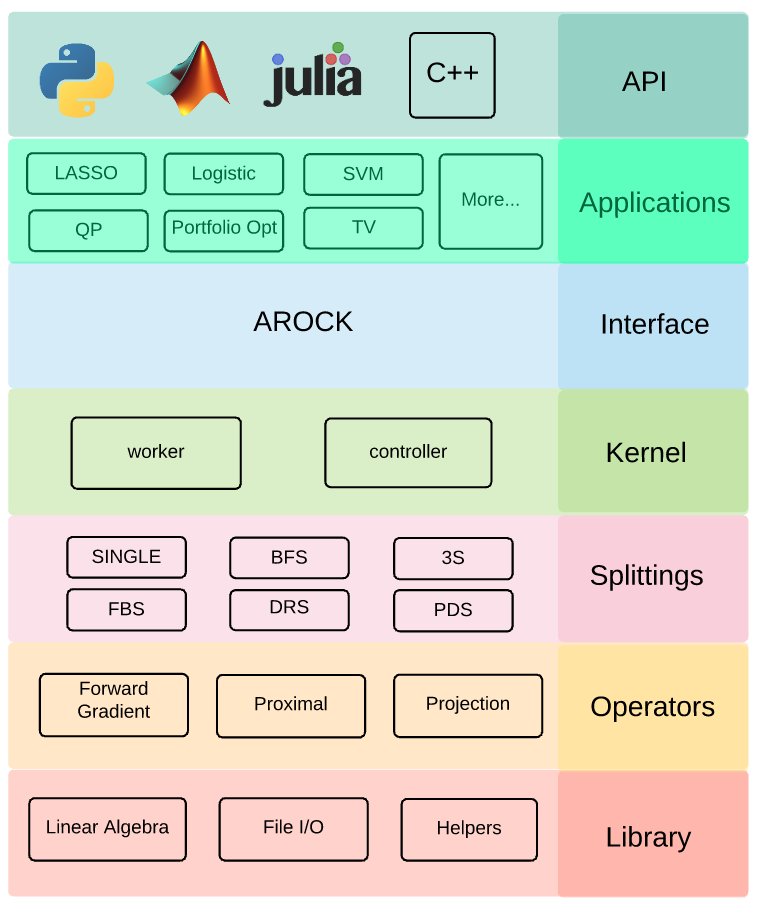
\includegraphics[width=0.48\textwidth]{./figs/architecture.png}
      \caption{Architectures for distributed memory systems.}
        \label{fig:arch}
\end{figure}


\subsection{Library}
The library layer includes three major components: linear algebra functions, wrappers and data structures, data file parsers, and helper functions. The major data structures are dense vector, dense matrix and sparse matrix. We implemented a few (Basic Linear Algebra Subprograms) BLAS level 1 and level 2 wrappers. File I/O functions for matrices in the matrix market format\footnote{http://math.nist.gov/MatrixMarket/formats.html} and LIBSVM format\footnote{https://www.csie.ntu.edu.tw/~cjlin/libsvmtools/datasets/} are also implemented. Helper functions include a list of objective function calculators, command argument parsers and error handling functions. 

\subsection{Operator}
The operator layer contains a library of projection operators, proximal operators and forward operators which implemented the operations required for a high-level iterative algorithm. These operators are implemented in the form of function object (functor). The following is a template for the operator functor. In general, each operator struct has three overloaded parenthesis operator: one takes a scalar; one takes a scalar and an index then applies the coordinate update; one takes an input vector and a output vector, then perform full update to the input vector and saves the results in the output vector. Default constructor and customized constructors are also provided. If an operator involves data, the point to the data should be added as a member variable. 

\begin{lstlisting}[language=c++]
  struct functor_name {
    // the step_size that associated with the operator  
    double step_size;
    // weight on the original function, e.g., f(x) = weight ||x||_1
    double weight;      
    // returns the operator evaluated on v at the given index
    double operator() (Vector* v, int index);
    // returns the operator evaluated on v at the given index
    double operator() (double val, int index);
    // full update
    void operator() (Vector* v_in, Vector* v_out);
    // (Optional) update the cached variables, it 
    // takes the old x_i and new x_i, updated at index.
    void update_cache_vars (double old_x_i, double new_x_i, int index);
    // update the step size. The step size might be
    // changed during the iterative process
    void update_step_size (double step_size_) {
      step_size = step_size_;
    }
    // customized constructor
    functor_name (double step_size_, double weight_ = 1.) :
        step_size(step_size_), weight(weight_) {}
    // default constructor
    functor_name () : step_size(0.), weight(1.) {}
  };
\end{lstlisting}

Currently, we implemented 17 operators, which are summarized in Table \ref{tab:prox}, Table \ref{tab:proj} and Table \ref{tab:forward}.
\begin{table}[htbp]
\centering
 \begin{tabular}{|c|c|c|}
  \hline
  Name & Definition & Proximal operator \\
  \hline
  \hline
  $\ell_1$ norm & $w \|x\|_1$ & $shrink(x, w \cdot \sigma)$ \\
  \hline  
  sum of squares & $\frac{w}{2} \|x\|_2^2$ & $\frac{1}{1 + w \cdot \sigma} x$ \\
  \hline 
  $\ell_2$ norm & $w \|x\|_2$ & $\begin{cases} 
  							0 & \text{ if } \|x\|_2 \leq w \sigma \\
							(1 - \frac{w \sigma}{\|x\|_2}) \cdot x & \text{otherwise}
							\end{cases}$ \\							
  \hline
  Huber function & $ \begin{cases}
  				\frac{w}{2} x^2, &\text{if} -\delta \leq x \leq \delta \\
				 w \delta(|x| - \frac{\delta}{2}), &\text{otherwise} \\
  			       \end{cases}$ & $\begin{cases} x -  w \sigma  \delta & \text{ if } x \geq \delta +  w \sigma \delta\\
			       \frac{x}{1 + \sigma w} & \text{ otherwise } \\
			        x +  w \sigma \delta  & \text{ if } x \leq -\delta -  w \sigma \delta\\
			       \end{cases}$ \\
  \hline		
 elastic net & $w_1 \|x\|_1 + \frac{w_2}{2} \|x\|_2^2$ &  $\frac{1}{1 + w_2 \sigma} \cdot shrink(x, w_1 \sigma)$\\
 \hline
 log barrier & $- w \sum_{i} \log(x_i)$ & $\frac{1}{2} (x_i + \sqrt{x_i^2 + 4 w \sigma}), \forall i$ \\
 \hline
 \end{tabular}
  \caption{Proximal operator.}
  \label{tab:prox}
\end{table}


\begin{table}[htbp]
\centering
 \begin{tabular}{|c|c|c|}
  \hline
  Name & Definition & Projection operator \\
  \hline
  \hline
  positive cone & $\{x ~|~ x \geq 0\}$ & $\max(0, x_i), \forall i$ \\
  \hline
  box & $\{x ~|~ l \leq x \leq u\}, l, u \in R^n$ & $\max(l_i, \min(x_i, u_i))$ \\
  \hline
  $\ell_1$ ball & $\{ x ~|~ \|x\|_1 \leq r \}$ & $O(n\log(n))$ method\\
  \hline 
  $\ell_2$ ball & $\{ x ~|~ \|x\|_2 \leq r \}$ & $\begin{cases} \frac{r}{\|x\|} \cdot x ~&\text{ if } \|x\|_2 \geq r \\
  										         x ~&\text{ otherwise }
  								   \end{cases} $\\
  \hline 
  hyperplane & $\{ x ~|~ a^T x = b \}$ & $x + \frac{(b - a^T x)}{a^Ta} \cdot a$\\
  \hline 
  probability simplex & $\{ x ~|~  x \geq 0, \sum_i x_i = 1\}$ & $O(n\log(n))$ method\\
  \hline   
 \end{tabular}
 \caption{Projection operator.}
   \label{tab:proj}
\end{table}


\begin{table}[htbp]
 \centering
 \begin{tabular}{|c|c|c|}
  \hline
  Name & Definition & Forward gradient operator \\
  \hline
  \hline
  square loss & $\frac{w}{2}\|A^Tx - b\|^2$ & $x - \sigma w A (A^T x - b)$ \\
  \hline
  quadratic function & $w (\frac{1}{2} x^T Q x + c^Tx + d)$ & $x - \sigma w (Q x + c)$ \\
  \hline
  logistic loss & $w \sum_i \log (1 + \exp(- b_i \cdot a_i^T x)) $ &  $x + \sigma w \sum_i \frac{b_i}{1 + \exp(b_i \cdot a_i^T x)} \cdot a_i$\\
  \hline
   square hinge loss & $\frac{w}{2} \sum \max(0, b_i (1 - a_i^T x))^2$ & $x +  \sigma w\sum b_i \max(0, b_i (1 - a_i^T x)) \cdot a_i$ \\
  \hline
   square huber loss & $w \sum huber(a_i^Tx - b_i)$ & $x  - \sigma  w \nabla huber(a_i^T x - b_i)$ \\
  \hline
 \end{tabular}
 \caption{Forward operator.} 
   \label{tab:forward}
\end{table}

\newpage
\subsection{Splitting Schemes}
Based on the discussions in Section \ref{sec:splitting}, we implemented several splitting schemes, including FBS, BFS and PRS. The structure of the splitting scheme has the following form. It usually has one or more than one operators as the template arguments. It has an overloaded parenthesis operator which performs updates to the unknown variable $x$ and maintained variables. 
 \begin{lstlisting}[language=c++]
 template <typename Op1, typename Op2, ...>
 struct OperatorSplitting {
   double relaxation_step_size;
   // update the unknown variable x at index
   // and also update the maintained variables   
   double operator(int index);
   // update the operator related parameters
   // and the relaxation parameter   
   void update_params(Params* params);
   // initialize the member variables with the input arguments
   OperatorSplitting(argument list);
};
\end{lstlisting}


\subsection{Worker, Controller and the ARock Interface}
In general, ARock consists of several workers and a controller. Each worker has access to the shared data, the maintained variables, the unknown parameter $x$, and other algorithm related constants. Each worker continuously updates some coordinates of $x$ until the stopping criterions are satisfied. At the same time, workers share delay monitoring information and convergence progress information with the controller, who use the information to dynamically update the step sizes to facilitate the convergence of ARock. The ARock interface simply spawns a set of threads with one thread taking the controller role and the rest of threads being the workers. 

\subsection{Applications}
We implemented several applications from statistical machine learning and scientific computing with the ARock framework. The applications can be compiled into executable files, which can then be executed through the command line interface. For an unimplemented application, if the necessary operators and splitting schemes are defined in the ARock library, then creating an async-parallel algorithm can be as simple as calling ARock on the splitting scheme.

